% This is samplepaper.tex, a sample chapter demonstrating the
% LLNCS macro package for Springer Computer Science proceedings;
% Version 2.21 of 2022/01/12
%
\documentclass[runningheads]{llncs}
%
\usepackage[T1]{fontenc}
% T1 fonts will be used to generate the final print and online PDFs,
% so please use T1 fonts in your manuscript whenever possible.
% Other font encondings may result in incorrect characters.
%
\usepackage{graphicx}
% Used for displaying a sample figure. If possible, figure files should
% be included in EPS format.
%
% If you use the hyperref package, please uncomment the following two lines
% to display URLs in blue roman font according to Springer's eBook style:
%\usepackage{color}
%\renewcommand\UrlFont{\color{blue}\rmfamily}
%\urlstyle{rm}
%
\begin{document}
%
\title{Schema Mechanisms as an Attempt to Implement Genetic Epistemology}
%
\titlerunning{Schema Mechanisms}
% If the paper title is too long for the running head, you can set
% an abbreviated paper title here
%
\author{Olivier L. Georgeon\inst{1}\orcidID{0000-0003-4883-8702} \and
Filipo Perotto\inst{2}\orcidID{1111-2222-3333-4444} \and
Third Author\inst{3}\orcidID{2222--3333-4444-5555}}
%
\authorrunning{O. Georgeon \& F. Perotto}
% First names are abbreviated in the running head.
% If there are more than two authors, 'et al.' is used.
%
\institute{UR CONFLUENCE: Sciences et Humanites (EA 1598), UCLy, France \email{ogeorgeon@univ-catholyon.fr}\\
	\and ONERA, France \email{filipo.perotto@onera.fr}
 \and
 }
%
\maketitle              % typeset the header of the contribution
%
\begin{abstract}
We review schema mechanisms as they have been used to account for a \textit{genetic} or \textit{constructivist} theory of learning.

\keywords{Schema mechanism  \and Genetic epistemology \and Constructivist learning.}
\end{abstract}
%
%
%
\section{Introduction}

\section{Genetic epistemology}

The notion of \textit{sensori-motor scheme} proposed by Piaget \cite{piaget_principles_1997}. 
Related to constructivist epistemology by \cite{glasersfeld_radical_1997}.


Piaget's genetic epistemology : 
``Knowledge does not originally arise either from a subject conscious of itself or from objects already constituted (from the subject's point of view) that would impose themselves on the subject. 
Knowledge results from interactions occurring halfway between the subject and the objects, and thus involving both, but due to a complete un-differentiation and not from exchanges between distinct forms.

If, at the beginning, there is neither a subject, in the epistemic sense of the term, nor objects, conceived as such, nor, above all, invariant instruments of exchange, then the initial problem of knowledge will be to construct such mediators. 
Starting from the contact zone between one's own body and the objects, these mediators will progressively engage more deeply in both complementary directions toward the exterior and the interior. 
It is from this dual progressive construction that the joint elaboration of both the subject and the objects depends.

The initial instrument of exchange is not perception, as rationalists too easily conceded to empiricism, but rather action itself, with its much greater plasticity. 
Certainly, perceptions play an essential role, but they partly depend on action as a whole, and some perceptual mechanisms that one might have thought to be innate or very primitive only emerge at a certain level of object construction.'' (translated from \cite{piaget_lepistemologie_2011}, p14-15)


Guerin and McKenzie \cite{guerin_survey_2013} proposed the graphical representation in Fig. \ref{fig:general}.

\begin{figure}
	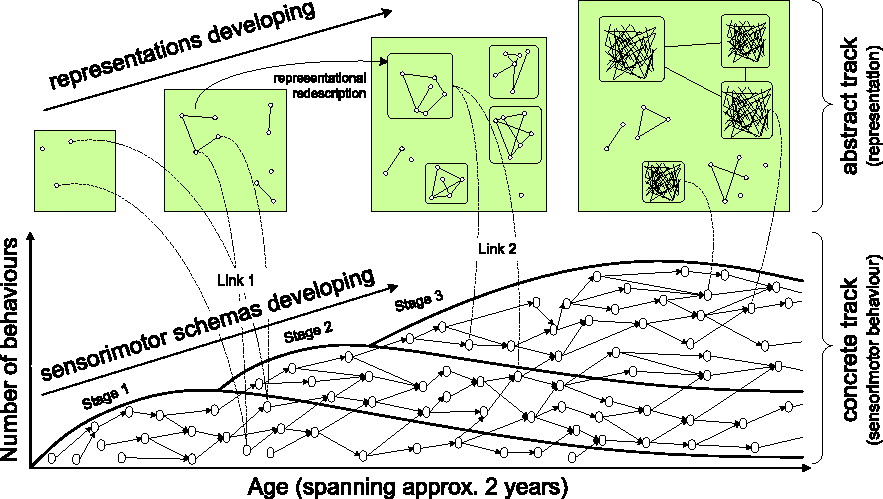
\includegraphics[width=\textwidth]{Figure_1_guerin.pdf}
	\caption{Conceptual diagram of infant development from \cite{guerin_survey_2013} Fig. 1.
	The lower (concrete) track shows a directed acyclic graph of sensorimotor schemas. 
	A node represents a newly created schema. 
	An edge has the meaning ``is a necessary precursor''. 
    Stage 1: behaviors without objects. 
    Stage 2: behaviors with single objects. 
    Stage 3: object-object behaviors. The schemas now involve relationship among objects, and locations and transforms within space.
    The higher (abstract) track represents representations of objects by schemas and physical properties influencing their interactions.} 
	\label{fig:general}
\end{figure}

Ziemke \cite{ziemke_construction_2001} examined how these views apply to robotics.


\section{Schema mechanisms}

Drescher \cite{drescher_made-up_1991} proposed the foundational schema mechanism by modeling schemas as depicted in Fig. \ref{fig:drescher}.

\begin{figure}
	\centering
	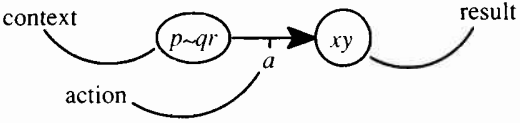
\includegraphics[width=0.6\textwidth]{Figure_2_schema_drescher.png}
	\caption{Schema from \cite{drescher_made-up_1991} Fig. 3.2.
	The schema noted $p \!\sim\! qr/a/xy$ asserts that if action $a$ is taken in the context where $p$ is true, $q$ is false, and $r$ is true then the resulting conditions $x$ and $y$ will be true.} 
	\label{fig:drescher}
\end{figure}

Bettoni  has criticized this model in stating that ``Drescher's Constructivism is not Piaget's Constructivism, mainly because of its tacit acceptance of \textit{cognitive dogmatism}'' (\cite{bettoni_made-up_1993}, p. 6).
He describes cognitive dogmatism as taking for granted that ``patterns and structures of objects, attributes, relations, etc. [...] be as much as possible true copies of 'original' objects, attributes, relations etc. in the world'' (\cite{bettoni_made-up_1993}, p. 1).
 
\cite{drescher_made-up_1991}
\cite{chaput_constructivist_2004}
\cite{georgeon_intrinsically-motivated_2012} 
\cite{perotto_computational_nodate} 
\cite{guerin_piagetian_2008}
\cite{wang_new_2012}
\section{Conclusion}

The problem of abstraction. 


\begin{credits}
\subsubsection{\ackname} .

\subsubsection{\discintname}
The authors have no competing interests to declare that are
relevant to the content of this article.
\end{credits}
%
% ---- Bibliography ----
%
% BibTeX users should specify bibliography style 'splncs04'.
% References will then be sorted and formatted in the correct style.
%
\bibliographystyle{splncs04}
\bibliography{ConstructivistAI.bib}
%
\end{document}
